\documentclass[a4paper]{scrartcl}

\usepackage{graphicx}
\usepackage[utf8]{inputenc}
\usepackage[bulgarian]{babel}
\usepackage{amsmath,amsfonts,amssymb,amsthm}
\usepackage{cwpuzzle}

\newcommand{\langdef}[5] { % {L}{w}{alphabet}{w math}{text} 
    \ensuremath{#1 = \left\{ #2 \in \{#3\}^* \mid #4 \right.} #5\ensuremath{\}.} 
}

\newcommand{\harder}{\emph{(по-трудна)}}

\title{Задачки-закачки 1}
\subtitle{ЕАИ-упражнения, групи 2 и 3}

\begin{document}

\maketitle

\centerline{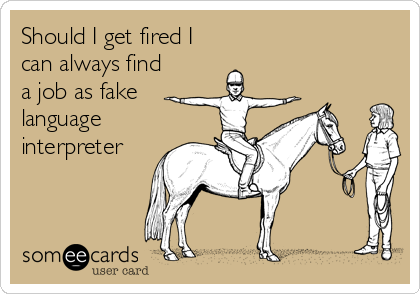
\includegraphics[scale=0.5]{eai}}

\begin{enumerate} 

    \section*{регулярни операции и регулярни изрази -- нормални задачки}

    \item За кои езици $L$, итерацията им $L^*$ е краен език?

    \item Намерете регулярен запис за езика $L$, където: 
        \begin{enumerate} 
            \item \langdef{L}{w}{0,1}{w}{е запис на число в двоична бройна система (без водещи нули!)}
                \emph{Решение:} $L = \{0\} \cup \left(\{1\} \cdot \{0, 1\}^*\right)$

            \item \langdef{L}{w}{0,1, \dots, 9}{w}{е запис на число в десетична бройна система, което се дели на 5, но не и на 25}

            \item \langdef{L}{w}{0,1,2}{w}{е запис на число в троична бройна система с дължина, деляща се на 3}

            \item \langdef{L}{w}{a}{|w| = 3x + 8y,}{за някои неотрицателни цели $x, y$, за които $x + y > 2$}

            \item \langdef{L}{w}{a,b,c}{w}{съдържа точно 3 пъти буквата $a$}

            \item \langdef{L}{w}{a,b,c}{w}{съдържа точно веднъж буквата $a$, точно два пъти буквата $b$ и точно три пъти буквата $c$}
        \end{enumerate}

    \item Намерете регулярен израз за езика: 
    \begin{enumerate}
        \item \langdef{L}{w}{a,b,c}{w}{има префикс $abc$ и суфикс $ca$}

            \item \langdef{L}{w}{a,b,c}{w}{не съдържа две последователни еднакви букви}

            \item \langdef{L}{w}{a,b,c}{w}{съдържа три последователни еднакви букви}

            \item \langdef{L}{w}{a,b,c}{w}{съдържа точно веднъж думата $bca$}

            \item \langdef{L}{w}{a,b}{}{в $w$ има поне две последователни букви $b$ след всяко срещане на буква $a$}

            \item \langdef{L}{w}{a,b}{w}{съдържа $ab$ и е с четна дължина}

            \item \langdef{L}{w}{a,b}{}{в $w$ има равен брой срещания на $ab$ и $ba$}

            \item \langdef{L}{w}{a,b}{}{в $w$ се срещат думите $ab$ и $ac$ и последното срещане на думата $ab$ е преди първото срещане на думата $ac$}

            \item \langdef{L}{w}{a,b}{w}{съдържа всяка възможна дума с дължина 2 точно по веднъж} \harder
        \end{enumerate}

    \item Напишете пълен регулярен израз над азбуката $\{a, b, c\}$ (без да има ... в него), който да се събира на един ред в тетрадката, който:
        \begin{enumerate}
            \item Разпознава точно 2 думи.
                \emph{Примерно решение:} \texttt{(a|b)}.
            \item Разпознава точно 9 думи, точно 27 думи, точно 81 думи.
            \item Разпознава точно 16 думи, точно 32 думи, точно 128 думи.
            \item Разпознава точно 63 думи, точно 64 думи, точно 65 думи.
        \end{enumerate}

    \section*{структурна индукция -- по-трудни задачки}

    \item Да се докаже, че обръщането $L^R$ на регулярен език $L$ е регулярен език.
        \begin{proof}[Доказателство.] За примитивните регулярни езици имаме $\{\}^R = \{\}, \{\epsilon\}^R = \{\epsilon\},
            \{a\}^R = \{a\}$, което показва, че са регулярни.  Нека $K^R$ е регулярен за произволен регулярен език $K$, имащ регулярен
            запис с по-малко от $k > 0$ прилагания на регулярните операции. 
        
            Нека $L$ е регулярен език, имащ регулярен запис с точно $k$ прилагания на регулярните операции. Възможни се следните случаи за $L$:
            \begin{itemize}
                \item $L = K_1 \cup K_2$, където $K_1$ и $K_2$ са регулярни и от индуктивното предположение $K_1^R$ и
                    $K_2^R$ също са регулярни. Тогава $L^R = (K_1 \cup K_2)^R = K_1^R \cup K_2^R$ е регулярен, защото е
                    обединение на регулярни езици.
                \item $L = K_1 K_2$, където $K_1$ и $K_2$ са регулярни и от индуктивното предположение $K_1^R$ и $K_2^R$
                    също са регулярни. Тогава $L^R = (K_1 K_2)^R = K_2^R K_1^R$ е регулярен, защото е конкатенация на
                    регулярни езици.
                \item $L = K^*$, където $K$ е регулярен и от индуктивното предположение $K^R$ също е регулярен. Тогава $L^R
                    = (K^*)^R = (K^R)^*$ е регулярен, защото е итерация на регулярен език.
            \end{itemize}
            Във всички възможни случаи за $L$ доказахме, че $L^R$ е регулярен.
            От това по индукция следва, че ако $L$ е регулярен, то и $L^R$ е регулярен.
        \end{proof}

    \item Нека $L \subseteq \{0, 1\}^*$ е регулярен език. Докажете, че следният език е регулярен:
        $L' = \{s(w), w \in L \mid s(w) = \text{разменяме нулите и единиците в } w\}$.

    \item Нека $L$ е регулярен език. Докажете, че ако удвоим всяка буква във всяка дума на $L$, новият език също е регулярен.

    \item Нека $L$ е регулярен език. Докажете, че езиците $L_{\text{even}}$, съставен от думите на $L$ с четна дължина и $L_{\text{odd}}$, съставен от думите на $L$ с нечетна дължина, са регулярни.

    \item Нека $A$ и $B$ са регулярни езици над една и съща азбука $\Sigma$. Перфектно картоподреждане $A \clubsuit B$ на $A$ и $B$ наричаме следния език:
        \[A \clubsuit B = \{ a_1 b_1 a_2 b_2 \dots a_k b_k \mid a_1 a_2 \dots a_k \in A, b_1 b_2 \dots b_k \in B, a_i \in \Sigma, b_i \in \Sigma\}.\]
        Да се докаже, че перфектното картоподреждане на два регулярни езика е регулярен език.

    \item Нека $L$ е регулярен език над азбуката $\Sigma$. Да се докаже, че перфектните картораздавания на $L$ са регулярни:
        \begin{align*}
            L_A &= \{a_1 a_2 \dots a_k \mid a_1 b_1 \dots a_k b_k \in L, a_i \in \Sigma, b_i \in \Sigma\}, \\
            L_B &= \{b_1 b_2 \dots b_k \mid a_1 b_1 \dots a_k b_k \in L, a_i \in \Sigma, b_i \in \Sigma\}.
        \end{align*}
    \item Нека $L$ е регулярен език. Да се докаже, че езикът $L_{\text{prefix}}$, образуван от префиксите на всички думи в $L$, e регулярен език.
        
\end{enumerate}

\section*{кръстословица}
\begin{Puzzle}{7}{6}
    |*   |[1]c|*   |[2]t|*   |*   |[3]a|.
    |[4]a|c   |c   |a   |c   |c   |c   |.
    |*   |c   |[5]b|a   |b   |a   |c   |.
    |[6]a|c   |t   |t   |t   |t   |t   |.
    |[7]c|c   |a   |t   |t   |t   |t   |.
    |*   |c   |*   |[8]a|c   |c   |c   |.
\end{Puzzle}
\begin{PuzzleClues}{\textbf{отвесно:}}
    \Clue{1}{cccccc}{\texttt{c(a*|c*)}}
    \Clue{2}{taatta}{\texttt{(at|ta)*}} \\
    \Clue{3}{accttc}{\texttt{a(a*c*t*)}}
\end{PuzzleClues}
\begin{PuzzleClues}{\textbf{водоравно:}}
    \Clue{4}{accaccc}{\texttt{ac*(a|b*)c*}}
    \Clue{5}{babac}{\texttt{(ba)*c}} \\
    \Clue{6}{acttttt}{\texttt{a(ba*|ct*)}}
    \Clue{7}{ccatttt}{\texttt{t*ac*|c*at*}}
    \Clue{8}{accc}{\texttt{a(b*|c*)}}
\end{PuzzleClues}
\end{document}
